\documentclass[10pt]{article}
\usepackage[letterpaper,text={6.5in,8.7in},centering]{geometry}
\usepackage{epic,eepic, pict2e}
\usepackage{amssymb,amsmath,times,subfigure,graphicx,theorem,tikz}
%\usepackage{amssymb,amsmath,times,url,subfigure,graphicx,theorem,alltt,eepic,tikz}

%\usepackage{warmread}
%\usepackage[all,import]{xy}
%\usepackage{eepic}

\newcommand{\norm}[1]{\ensuremath{\left\| #1 \right\|}}
\newcommand{\abs}[1]{\ensuremath{\left| #1 \right|}}
\newcommand{\bracket}[1]{\ensuremath{\left[ #1 \right]}}
\newcommand{\braces}[1]{\ensuremath{\left\{ #1 \right\}}}
\newcommand{\parenth}[1]{\ensuremath{\left( #1 \right)}}
\newcommand{\ip}[1]{\ensuremath{\langle #1 \rangle}}
\newcommand{\refeqn}[1]{(\ref{eqn:#1})}
\newcommand{\reffig}[1]{Fig. \ref{fig:#1}}
\newcommand{\tr}[1]{\mbox{tr}\ensuremath{\negthickspace\bracket{#1}}}
\newcommand{\deriv}[2]{\ensuremath{\frac{\partial #1}{\partial #2}}}
\newcommand{\SO}{\ensuremath{\mathrm{SO(3)}}}
\newcommand{\T}{\ensuremath{\mathrm{T}}}
\newcommand{\so}{\ensuremath{\mathfrak{so}(3)}}
\newcommand{\SE}{\ensuremath{\mathrm{SE(3)}}}
\newcommand{\se}{\ensuremath{\mathfrak{se}(3)}}
\renewcommand{\Re}{\ensuremath{\mathbb{R}}}
\renewcommand{\S}{\ensuremath{\mathbb{S}}}
\newcommand{\aSE}[2]{\ensuremath{\begin{bmatrix}#1&#2\\0&1\end{bmatrix}}}
\newcommand{\ase}[2]{\ensuremath{\begin{bmatrix}#1&#2\\0&0\end{bmatrix}}}
\newcommand{\D}{\ensuremath{\mathbf{D}}}
\newcommand{\pair}[1]{\ensuremath{\left\langle #1 \right\rangle}}
\newcommand{\met}[1]{\ensuremath{\langle\!\langle #1 \rangle\!\rangle}}
\newcommand{\Ad}{\ensuremath{\mathrm{Ad}}}
\newcommand{\ad}{\ensuremath{\mathrm{ad}}}
\newcommand{\g}{\ensuremath{\mathfrak{g}}}

\renewcommand{\baselinestretch}{1.2}
\date{}

\renewcommand{\thesubsection}{\arabic{subsection}. }
\renewcommand{\thesubsubsection}{\arabic{subsection}.\arabic{subsubsection} }

\theoremstyle{plain}\theorembodyfont{\normalfont}
\newtheorem{prob}{Problem}[section]
%\renewcommand{\theprob}{\arabic{section}.\arabic{prob}}
\renewcommand{\theprob}{\arabic{prob}}

\newenvironment{subprob}%
{\renewcommand{\theenumi}{\alph{enumi}}\renewcommand{\labelenumi}{(\theenumi)}\begin{enumerate}}%
{\end{enumerate}}%

\newcommand*\circled[1]{%
  \tikz[baseline=(C.base)]\node[draw,circle,inner sep=0.5pt](C) {#1};\!
}


\begin{document}

\vspace*{1cm}

\pagestyle{empty}
\centerline{\LARGE{ MAE3145: Final Exam}}
\vspace*{0.5cm}
\centerline{\Large December 14, 2016}%\\%\vspace*{0.5cm}

\vspace*{6cm}

\centerline{
\begin{tabular}{lll}
\hspace*{5cm}, & \hspace*{5cm}. & \hspace*{4cm}\\\hline
Last Name & First Name & Student ID
\end{tabular}}

\vspace*{6cm}

\centerline{
\begin{tabular}{|c|c|c|c|c|c|c|}\hline
Prob. 1 & Prob. 2 & Prob. 3 & Prob. 4 & Prob. 5 & Total \\
(20) & (15) & (20) & (15) & (10) & (80)\\ \hline
\hspace*{2.cm} & \hspace*{2.cm} & \hspace*{2.cm} & \hspace*{2.cm} & \hspace*{2.cm} & \hspace*{2.2cm} \\
&&&&&\\
&&&&&\\\hline
\end{tabular}}

\renewcommand{\thepage}{\arabic{page}/8}
\clearpage\newpage\setcounter{page}{1}\pagestyle{plain}

\renewcommand{\theprob}{\arabic{prob} \textit{(20pt)}}
\begin{prob}
Mark whether each statement written in \textit{italic font} is True or False.% (for (a)-(d)), or answer the question shortly (for (e)).

\begin{subprob}
%\item \textit{The orbital period of the Mars is greater than the orbital period of the Saturn}. [True, False]
%\vspace*{1.2cm}

\item The orbital radius of the Earth is $149.6\times 10^6\,\mathrm{km}$, and the orbital radius of the Jupiter is $778.6\times 10^6\,\mathrm{km}$. \textit{The standard Hohmann transfer from the Earth to the Jupiter is always more efficient that the bi-elliptic Hohmann transfer between them.} [True, False]

\item Spacecraft $A$ and $B$ are on the same orbit. The chaser spacecraft $A$ executes a phasing maneuver to catch the target spacecraft $B$ after one revolution at the point $A$. \textit{Then, the chaser spacecraft $A$ should increase its velocity at the beginning of the phasing maneuver.} [True, False] 

    \begin{figure}[htbp]
        \centering
        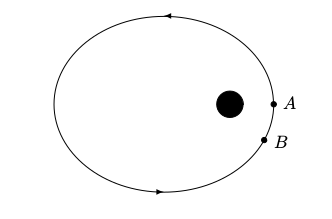
\includegraphics[width=0.5\textwidth]{figures/prob1.png}
    \end{figure}

%\item We wish to transfer a spacecraft from the inner elliptic orbit to the outer elliptic orbit using a Hohmann transfer. \textit{The Hohmann transfer from $A$ to $B$ is more efficient than the Hohmann transfer from $A'$ to $B'$.} [True, False]
%
%\centerline{
%\setlength{\unitlength}{2.5em}\centering
%\begin{picture}(6,5.5)(-3.0,-3)
%\put(1.5,0){\circle*{0.6}}
%\put(-0.5,0){\ellipse{7.0}{4.0}}
%\put(0.5,0){\ellipse{4.0}{2.4}}
%\put(2.5,0){\circle*{0.12}}
%\put(-1.5,0){\circle*{0.12}}
%\put(3,0){\circle*{0.12}}
%\put(-4,0){\circle*{0.12}}
%\put(2.5,-0.3){$A$}
%\put(-4.5,-0.3){$B$}
%\put(-2.1,-0.3){$A'$}
%\put(3.1,-0.3){$B'$}
%\put(-0.5,2){\vector(-1,0){0.0}}
%\put(-0.5,-2){\vector(1,0){0.0}}
%\put(0.5,1.2){\vector(-1,0){0.0}}
%\put(0.5,-1.2){\vector(1,0){0.0}}
%\end{picture}}


%\item A spacecraft is on an elliptic orbit. When it passes through the periapsis $P$, its rocket is fired along the outward radial direction as shown below. Then, \textit{the eccentricity vector $\vec e$ rotates clockwise}. [True, False]
%
%\centerline{
%\setlength{\unitlength}{2.5em}\centering
%\begin{picture}(6,4.5)(-3,-2.5)
%\put(1.5,0){\circle*{0.6}}
%\put(-0.4,0){\ellipse{6.0}{3.0}}
%\put(2.6,0){\circle*{0.12}}
%\put(2.6,0){\vector(1,0){1.2}}
%\put(2.7,-0.4){$P$}
%\put(-0.4,1.5){\vector(-1,0){0.0}}
%\put(-0.4,-1.5){\vector(1,0){0.0}}
%\end{picture}}
%
%
%
%\item A spacecraft is on a circular orbit around the Earth. \textit{Escaping from the Earth gravitational field completely requires a larger velocity increment than rotating its orbital plane by $30^\circ$ without changing the orbital shape and size}. [True, False]
%
%%
%%\item The ground tracks for two spacecraft are illustrated as follows. \textit{The inclination of Spacecraft 1 is greater than Spacecraft 2, i.e. $i_1> i_2$}. [True, False]
%%
%%\centerline{
%%\setlength{\unitlength}{0.1\textwidth}\centering
%%\begin{picture}(6,3.2)(0,0)\footnotesize
%%\put(0,0){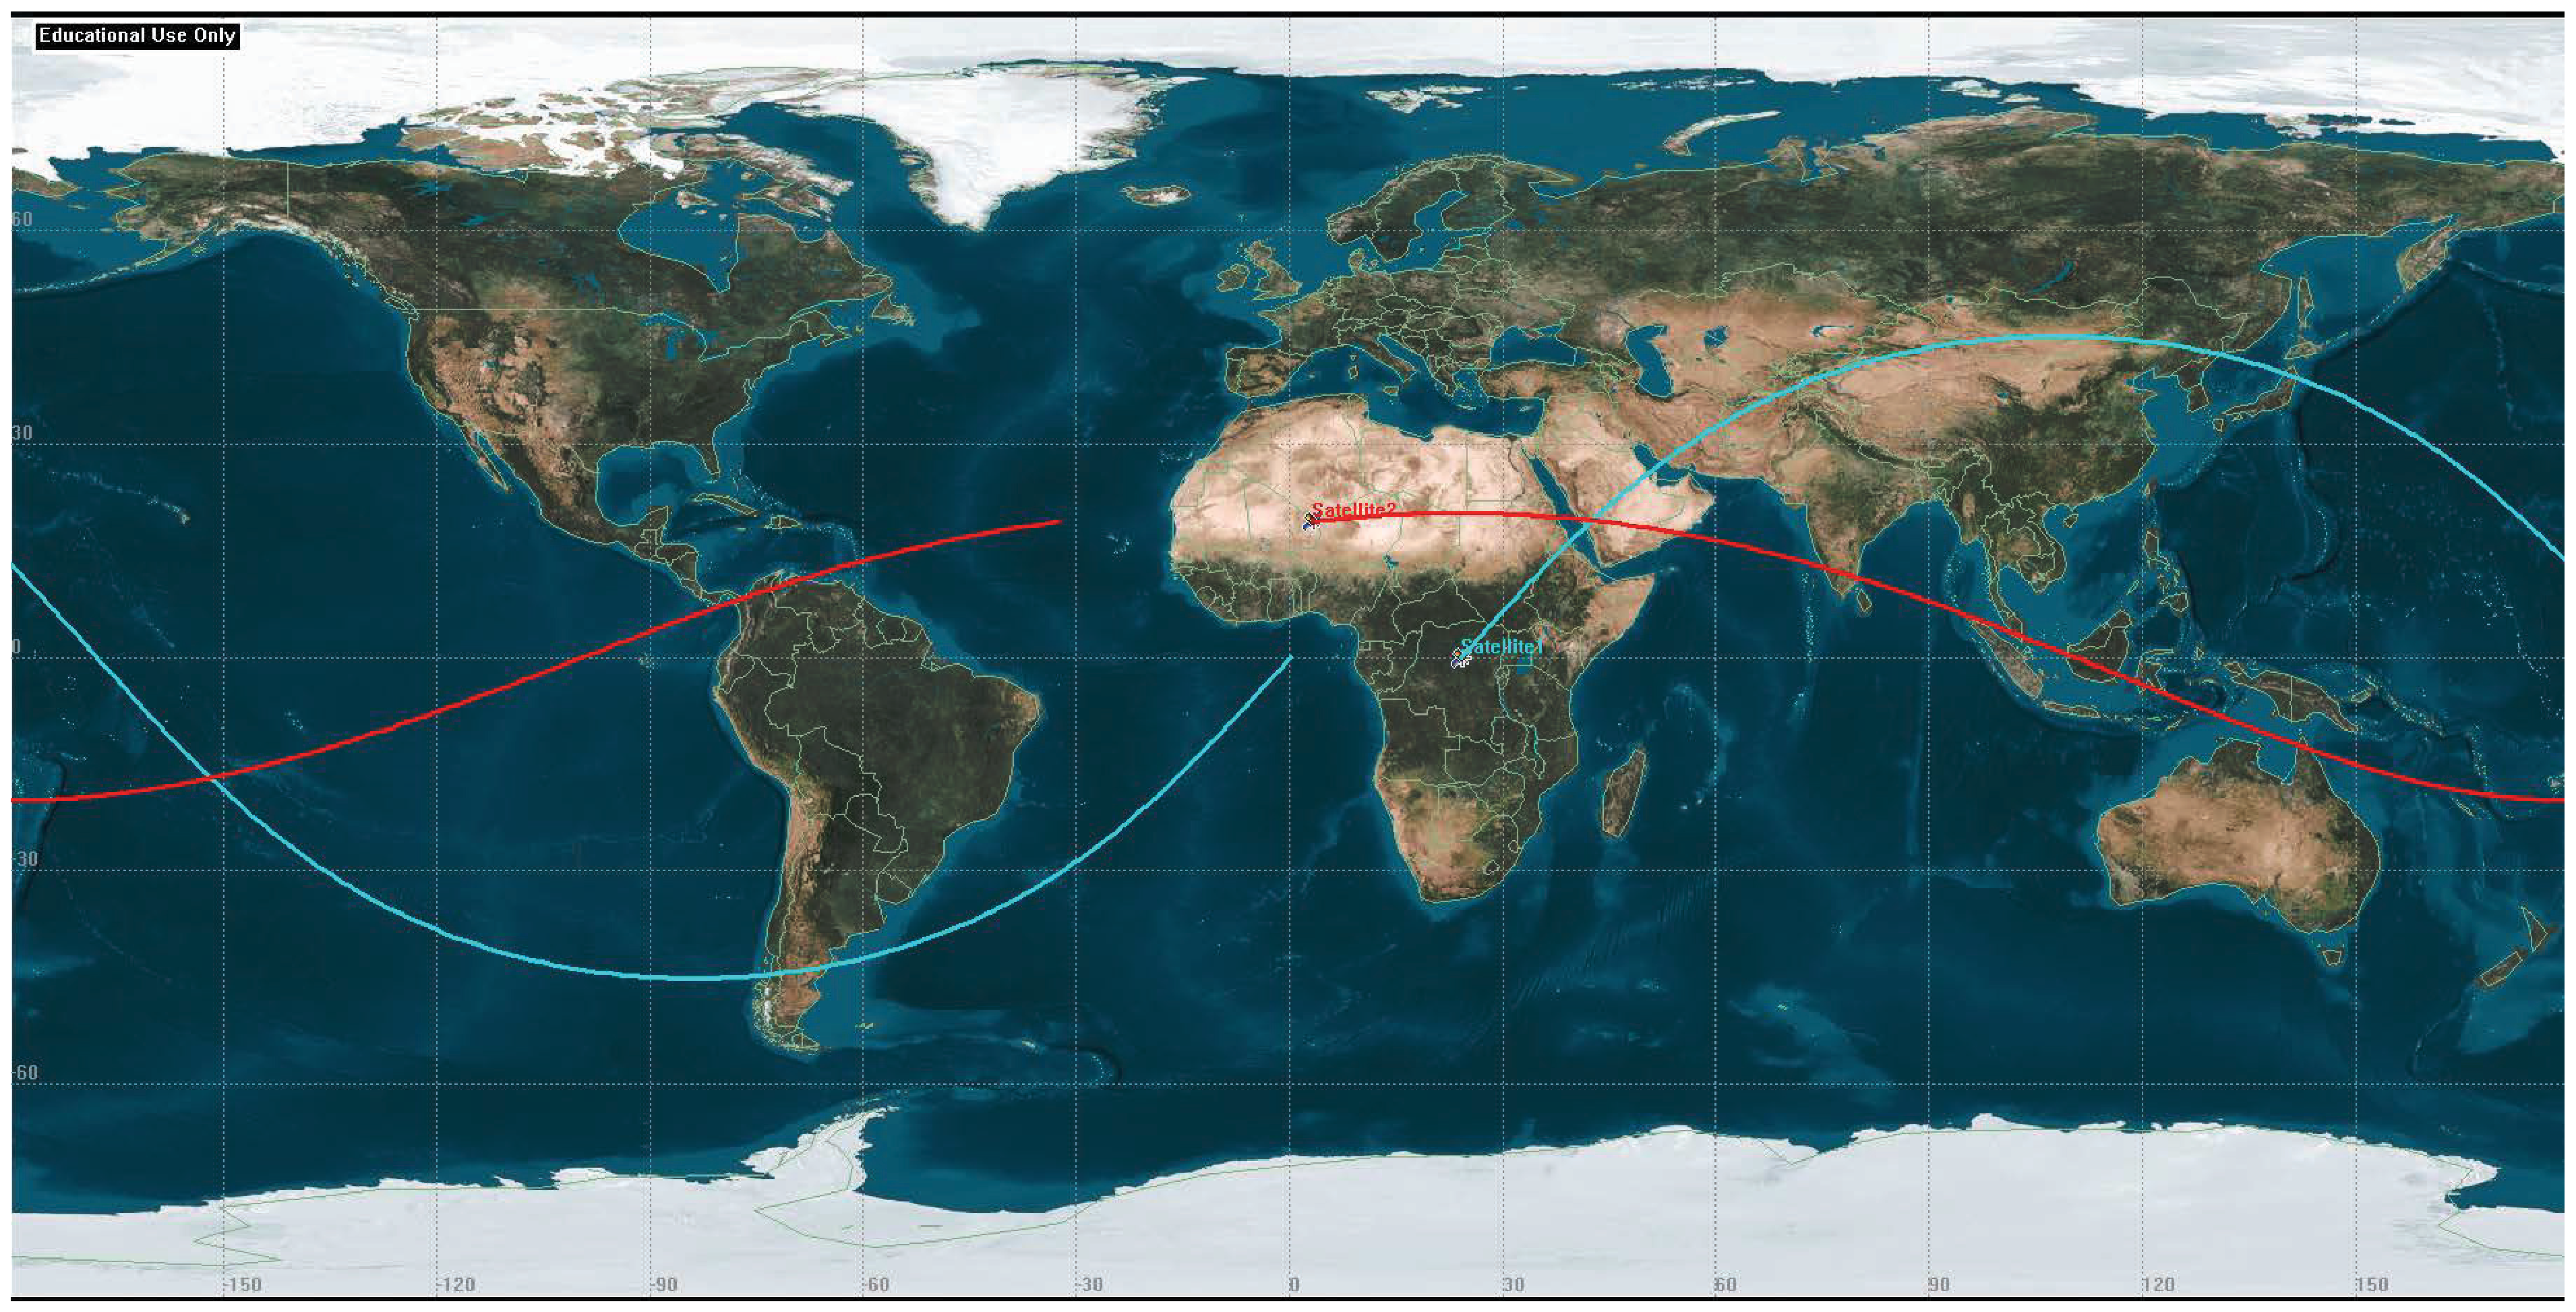
\includegraphics[width=0.6\textwidth]{Prob1.eps}}
%%\put(6.1,1.7){Spacecraft 1 (blue)}
%%\put(6.1,1.05){Spacecraft 2 (red)}
%%\end{picture}}
%
%
%\item \textit{Among the five Lagrange points in the Earth-Moon system, the first Lagrange point $L_1$ has the lowest value of the Jacobi constant, i.e. $L_1$ has the minimum energy.} [True, False]
%
%\item Kennedy Space Center has been NASA's primary launch center of human spaceflight since December 1968. Describe \textit{shortly} one of the \textit{engineering} benefits of locating a lauch center in the southern east coast, compared with other places like Portland, OR. (Please, exclude political or climate-related issues.)


%\item \textit{Among the five Lagrange points in the Earth-Moon system, the first Lagrange point $L_1$ has the lowest value of the Jacobi constant, i.e. $L_1$ has the minimum energy.} [True, False]

\item Consider a satellite on a circular orbit around the Earth. \textit{Changing the orbital inclination by $15^\circ$ requires more $\Delta v$ than that to make it completely escape from the Earth gravitational field.} [True, False] 



\end{subprob}
\end{prob}



%\clearpage\newpage

%\begin{prob}
%A spacecraft is on a circular orbit with orbital velocity $v_\circ$. 

%\begin{subprob}
%\item Show that the velocity change $\Delta v_h$ required to transfer the spacecraft into a hyperbolic orbit with eccentricity $e$ is given by
%\begin{align*}
%\Delta v_{h} = v_{\circ} (\sqrt{1+e} -1).
%\end{align*}
%\vspace*{6cm}
%\item 
%\end{subprob}

%\end{prob}


\clearpage\newpage
\renewcommand{\theprob}{\arabic{prob} \textit{(15pt)}}
\begin{prob}
Spacecraft $A$ is on a circular orbit \circled{1} around the Earth, and Spacecraft $B$ is on an elliptic orbit \circled{2} around the Earth.

\begin{figure}[htbp]
    \centering
    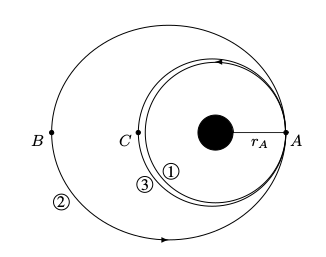
\includegraphics[width=0.5\textwidth]{figures/prob3.png}
\end{figure}
\begin{align*}
\mu = 398600\,\mathrm{km^3/s^2},\qquad r_A=8000\,\mathrm{km},\qquad e_2 = 0.4.
\end{align*}

\noindent We wish to design a phase maneuver of Spacecraft $A$ such that rendezvous between Spacecraft $A$ and $B$ occurs at the point $A$ after one revolution. After the rendezvous, Spacecraft $A$ is transferred to Orbit \circled{2}. Let Orbit \circled{3} be the phasing orbit of Spacecraft $A$, and let $C$ be the apoapsis of Orbit \circled{3}.

\begin{subprob}
\item Find the time $t_{BA}$ for Spacecraft B to return to the point $A$.
\vspace*{6cm}
\item Find the period $T_3$ and the apoapsis distance $r_C$ of the phasing orbit \circled{3}.
\newpage
\item Find the velocity change $\Delta v_A = v_{A_3}-v_{A_1}$ at the beginning of the phasing maneuver.
\vspace*{6cm}
\item Find the velocity change $\Delta v_{A'} = v_{A_2}-v_{A_3}$ at the end of the phasing maneuver.
\vspace*{6cm}
\item Show that the total velocity change to complete the phasing maneuver is $1.2933\,\mathrm{km/s}$.

\end{subprob} 
 
\end{prob}





\clearpage\newpage
\renewcommand{\theprob}{\arabic{prob} \textit{(20pt)}}
\begin{prob}
Consider a spacecraft on a circular orbit with radius $r_P$. We wish to rotate the orbital plane by $\delta$ without changing the orbit shape and size. In the class, we found that the required velocity change for one-impulse plane change maneuver is given by
\begin{align}
\Delta v = 2v\sin\frac{\delta}{2},\qquad \text{where }\quad v=\sqrt{\frac{\mu}{r_P}}.\label{eqn:delVoim}
\end{align}
This cost of a plane change is quite high. In this question, we try to reduce the cost of a plane change by designing a series of maneuvers. Let the initial circular orbit be denoted by \circled{1}, and the terminal rotated circular orbit be \circled{4}. The proposed maneuver from \circled{1} to \circled{4} is composed of the following three steps:

\begin{list}{$-$}{\setlength{\itemsep}{0pt}}
\item \circled{1}$\rightarrow$\circled{2} at $P$: transfer the spacecraft to an elliptic orbit \circled{2},
\item \circled{2}$\rightarrow$\circled{3} at $A$: perform a plane change maneuver at the apoapsis $A$ of the elliptic orbit \circled{2},
%\item \circled{2}$\rightarrow$\circled{3} at $A$: transfer the spacecraft back to the periapsis $P$ on the rotated elliptic orbit \circled{3},
\item \circled{3}$\rightarrow$\circled{4} at $P$: transfer the spacecraft to the rotated circular orbit \circled{4} at the periapsis $P$.
\end{list}
Let the apoapsis distance of the transferring elliptic orbits be $r_A>r_P$. These orbits are illustrated as follows:

\begin{figure}[htbp]
    \centering
    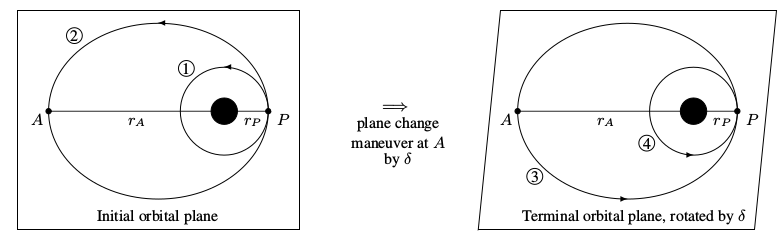
\includegraphics[width=0.9\textwidth]{figures/prob4.png}
\end{figure}

\begin{center}\vspace*{0.1cm}
{\small\selectfont
\begin{tabular}{|c|c|c|c|c|c|c|c|}\hline
& Description  & Inclination & Periapsis & Apoapsis & Velocity at the beginning & Velocity at the end\\\hline
Orbit \circled{1} & Initial circular orbit & 0 & $r_P$ & $r_P$ & $V_{P_1}$ & - \\
Orbit \circled{2} & Hohmann transfer orbit & 0 & $r_P$ & $r_A$ & $V_{P_2}$ & $V_{A_2}$ \\
Orbit \circled{3} & Hohmann transfer orbit & $\delta$ & $r_P$ & $r_A$ & $V_{A_3}$ & $V_{P_3}$ \\
Orbit \circled{4} & Target circular orbit & $\delta$ & $r_P$ & $r_P$ & $V_{P_4}$ & - \\\hline
\end{tabular}}
\end{center}

\begin{subprob}
\item Find $\Delta v_P$ to transfer the spacecraft from the initial circular orbit \circled{1} to the  elliptic orbit \circled{2} at $P$.
\vspace*{3.5cm}

\item Find $\Delta v_A$ required to rotate the orbital plane of Orbit \circled{2} by $\delta$ at $A$, transferring the spacecraft to Orbit \circled{3}.
\vspace*{3.5cm}

\item Find $\Delta v_{P'}$ to transfer the spacecraft from the  elliptic orbit \circled{3} to the terminal circular orbit \circled{4} at $P$.
\vspace*{3cm}

%\newpage
\item The ratio of the total velocity change $\Delta v_T=|\Delta v_P| + |\Delta v_A| + |\Delta v_{P'}|$ of this maneuver to the velocity change $\Delta v$ of the one-impulse maneuver at \refeqn{delVoim} can be written as
\begin{align}
%\frac{\Delta v_T}{\Delta v} = \sqrt{\frac{2}{\rho(1+\rho)}} + \frac{1}{\sin \delta/2}\bracket{\sqrt{\frac{2\rho}{1+\rho}}-1},\label{eqn:VTV}
\frac{\Delta v_T}{\Delta v} = \sqrt{\frac{2}{\rho(1+\rho)}} + \frac{1}{\sin \delta/2}\bigg\{\hspace*{2cm}\bigg\},\label{eqn:VTV}
\end{align}
where $\rho=\dfrac{r_A}{r_P}>1$. Find the expression in the braces $\{\;\}$.\; (Hint: $|\Delta v_{P'}| = |\Delta v_{P}|$).
\vspace*{7cm}

%\textcolor{red}{Maybe, show only parts of (2)}

\item Suppose that $\rho=2$, and $\delta=60^\circ$. Using \refeqn{VTV}, determine which is more energy efficient between the proposed three-impulse maneuver with the cost of $\Delta v_T$, and the one-impulse maneuver with the cost of $\Delta v$. 

\end{subprob}

\end{prob}



\clearpage\newpage
\renewcommand{\theprob}{\arabic{prob} \textit{(15pt)}}
\begin{prob}
The international Cassini mission to the Saturn made use of gravity assist from the Venus. In this question, we develop the rendezvous condition for a Hohmann transfer from the Earth to the Venus. The locations of the Earth and the Venus at the departure and the arrival are illustrated as follows.

\begin{figure}[htbp]
    \centering
    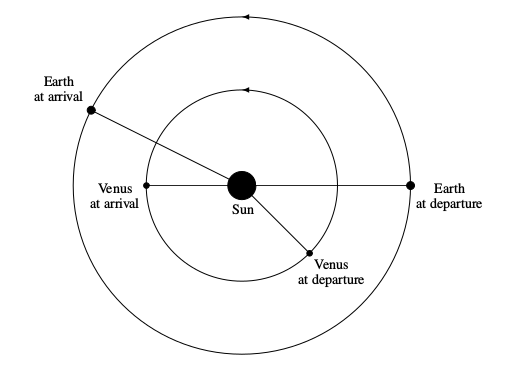
\includegraphics[width=0.6\textwidth]{figures/prob5.png}
\end{figure}

\begin{align*}
\mu_S = 1.327\times 10^{11}\,\mathrm{km^3/s^2},\qquad R_E=149.6\times 10^6\,\mathrm{km},\qquad R_V=108.2\times 10^6\,\mathrm{km}.
\end{align*}

\begin{subprob}
\item Find the travel time $t_{EV}$ from the Earth to the Venus along the Hohmann transfer orbit between them.
\vspace*{4cm}
\item Let $\phi$ be the phase angle of the Venus relative to the Earth, i.e. $\phi=\theta_V-\theta_E$, and let $\phi_0$ be the value of the phase angle at departure. The rotation angle of the Venus during the Hohmann transfer is given by $n_V t_{EV}$. Mark the angles $\phi_0$ and $n_V t_{EV}$ in the above diagram.
\item Find $\phi_0$ for a rendezvous between the Venus and the spacecraft to occur at the end of the Hohmann transfer. (Hint: $\phi_0<0$)
\end{subprob}

\end{prob}




\end{document}

